\title{A Very Simple \LaTeXe{} Template}
\author{
        Vitaly Surazhsky \\
                Department of Computer Science\\
        Technion---Israel Institute of Technology\\
        Technion City, Haifa 32000, \underline{Israel}
            \and
        Yossi Gil\\
        Department of Computer Science\\
        Technion---Israel Institute of Technology\\
        Technion City, Haifa 32000, \underline{Israel}
}
\date{\today}

\documentclass[12pt]{article}

\usepackage{makeidx}
\makeindex

%\documentclass{article}
\usepackage{fancyvrb}
\usepackage{color}
%\usepackage[utf-8]{inputenc}



\makeatletter
\def\PY@reset{\let\PY@it=\relax \let\PY@bf=\relax%
    \let\PY@ul=\relax \let\PY@tc=\relax%
    \let\PY@bc=\relax \let\PY@ff=\relax}
\def\PY@tok#1{\csname PY@tok@#1\endcsname}
\def\PY@toks#1+{\ifx\relax#1\empty\else%
    \PY@tok{#1}\expandafter\PY@toks\fi}
\def\PY@do#1{\PY@bc{\PY@tc{\PY@ul{%
    \PY@it{\PY@bf{\PY@ff{#1}}}}}}}
\def\PY#1#2{\PY@reset\PY@toks#1+\relax+\PY@do{#2}}

\def\PY@tok@gd{\def\PY@tc##1{\textcolor[rgb]{0.63,0.00,0.00}{##1}}}
\def\PY@tok@gu{\let\PY@bf=\textbf\def\PY@tc##1{\textcolor[rgb]{0.50,0.00,0.50}{##1}}}
\def\PY@tok@gt{\def\PY@tc##1{\textcolor[rgb]{0.00,0.25,0.82}{##1}}}
\def\PY@tok@gs{\let\PY@bf=\textbf}
\def\PY@tok@gr{\def\PY@tc##1{\textcolor[rgb]{1.00,0.00,0.00}{##1}}}
\def\PY@tok@cm{\let\PY@it=\textit\def\PY@tc##1{\textcolor[rgb]{0.25,0.50,0.50}{##1}}}
\def\PY@tok@vg{\def\PY@tc##1{\textcolor[rgb]{0.10,0.09,0.49}{##1}}}
\def\PY@tok@m{\def\PY@tc##1{\textcolor[rgb]{0.40,0.40,0.40}{##1}}}
\def\PY@tok@mh{\def\PY@tc##1{\textcolor[rgb]{0.40,0.40,0.40}{##1}}}
\def\PY@tok@go{\def\PY@tc##1{\textcolor[rgb]{0.50,0.50,0.50}{##1}}}
\def\PY@tok@ge{\let\PY@it=\textit}
\def\PY@tok@vc{\def\PY@tc##1{\textcolor[rgb]{0.10,0.09,0.49}{##1}}}
\def\PY@tok@il{\def\PY@tc##1{\textcolor[rgb]{0.40,0.40,0.40}{##1}}}
\def\PY@tok@cs{\let\PY@it=\textit\def\PY@tc##1{\textcolor[rgb]{0.25,0.50,0.50}{##1}}}
\def\PY@tok@cp{\def\PY@tc##1{\textcolor[rgb]{0.74,0.48,0.00}{##1}}}
\def\PY@tok@gi{\def\PY@tc##1{\textcolor[rgb]{0.00,0.63,0.00}{##1}}}
\def\PY@tok@gh{\let\PY@bf=\textbf\def\PY@tc##1{\textcolor[rgb]{0.00,0.00,0.50}{##1}}}
\def\PY@tok@ni{\let\PY@bf=\textbf\def\PY@tc##1{\textcolor[rgb]{0.60,0.60,0.60}{##1}}}
\def\PY@tok@nl{\def\PY@tc##1{\textcolor[rgb]{0.63,0.63,0.00}{##1}}}
\def\PY@tok@nn{\let\PY@bf=\textbf\def\PY@tc##1{\textcolor[rgb]{0.00,0.00,1.00}{##1}}}
\def\PY@tok@no{\def\PY@tc##1{\textcolor[rgb]{0.53,0.00,0.00}{##1}}}
\def\PY@tok@na{\def\PY@tc##1{\textcolor[rgb]{0.49,0.56,0.16}{##1}}}
\def\PY@tok@nb{\def\PY@tc##1{\textcolor[rgb]{0.00,0.50,0.00}{##1}}}
\def\PY@tok@nc{\let\PY@bf=\textbf\def\PY@tc##1{\textcolor[rgb]{0.00,0.00,1.00}{##1}}}
\def\PY@tok@nd{\def\PY@tc##1{\textcolor[rgb]{0.67,0.13,1.00}{##1}}}
\def\PY@tok@ne{\let\PY@bf=\textbf\def\PY@tc##1{\textcolor[rgb]{0.82,0.25,0.23}{##1}}}
\def\PY@tok@nf{\def\PY@tc##1{\textcolor[rgb]{0.00,0.00,1.00}{##1}}}
\def\PY@tok@si{\let\PY@bf=\textbf\def\PY@tc##1{\textcolor[rgb]{0.73,0.40,0.53}{##1}}}
\def\PY@tok@s2{\def\PY@tc##1{\textcolor[rgb]{0.73,0.13,0.13}{##1}}}
\def\PY@tok@vi{\def\PY@tc##1{\textcolor[rgb]{0.10,0.09,0.49}{##1}}}
\def\PY@tok@nt{\let\PY@bf=\textbf\def\PY@tc##1{\textcolor[rgb]{0.00,0.50,0.00}{##1}}}
\def\PY@tok@nv{\def\PY@tc##1{\textcolor[rgb]{0.10,0.09,0.49}{##1}}}
\def\PY@tok@s1{\def\PY@tc##1{\textcolor[rgb]{0.73,0.13,0.13}{##1}}}
\def\PY@tok@sh{\def\PY@tc##1{\textcolor[rgb]{0.73,0.13,0.13}{##1}}}
\def\PY@tok@sc{\def\PY@tc##1{\textcolor[rgb]{0.73,0.13,0.13}{##1}}}
\def\PY@tok@sx{\def\PY@tc##1{\textcolor[rgb]{0.00,0.50,0.00}{##1}}}
\def\PY@tok@bp{\def\PY@tc##1{\textcolor[rgb]{0.00,0.50,0.00}{##1}}}
\def\PY@tok@c1{\let\PY@it=\textit\def\PY@tc##1{\textcolor[rgb]{0.25,0.50,0.50}{##1}}}
\def\PY@tok@kc{\let\PY@bf=\textbf\def\PY@tc##1{\textcolor[rgb]{0.00,0.50,0.00}{##1}}}
\def\PY@tok@c{\let\PY@it=\textit\def\PY@tc##1{\textcolor[rgb]{0.25,0.50,0.50}{##1}}}
\def\PY@tok@mf{\def\PY@tc##1{\textcolor[rgb]{0.40,0.40,0.40}{##1}}}
\def\PY@tok@err{\def\PY@bc##1{\fcolorbox[rgb]{1.00,0.00,0.00}{1,1,1}{##1}}}
\def\PY@tok@kd{\let\PY@bf=\textbf\def\PY@tc##1{\textcolor[rgb]{0.00,0.50,0.00}{##1}}}
\def\PY@tok@ss{\def\PY@tc##1{\textcolor[rgb]{0.10,0.09,0.49}{##1}}}
\def\PY@tok@sr{\def\PY@tc##1{\textcolor[rgb]{0.73,0.40,0.53}{##1}}}
\def\PY@tok@mo{\def\PY@tc##1{\textcolor[rgb]{0.40,0.40,0.40}{##1}}}
\def\PY@tok@kn{\let\PY@bf=\textbf\def\PY@tc##1{\textcolor[rgb]{0.00,0.50,0.00}{##1}}}
\def\PY@tok@mi{\def\PY@tc##1{\textcolor[rgb]{0.40,0.40,0.40}{##1}}}
\def\PY@tok@gp{\let\PY@bf=\textbf\def\PY@tc##1{\textcolor[rgb]{0.00,0.00,0.50}{##1}}}
\def\PY@tok@o{\def\PY@tc##1{\textcolor[rgb]{0.40,0.40,0.40}{##1}}}
\def\PY@tok@kr{\let\PY@bf=\textbf\def\PY@tc##1{\textcolor[rgb]{0.00,0.50,0.00}{##1}}}
\def\PY@tok@s{\def\PY@tc##1{\textcolor[rgb]{0.73,0.13,0.13}{##1}}}
\def\PY@tok@kp{\def\PY@tc##1{\textcolor[rgb]{0.00,0.50,0.00}{##1}}}
\def\PY@tok@w{\def\PY@tc##1{\textcolor[rgb]{0.73,0.73,0.73}{##1}}}
\def\PY@tok@kt{\def\PY@tc##1{\textcolor[rgb]{0.69,0.00,0.25}{##1}}}
\def\PY@tok@ow{\let\PY@bf=\textbf\def\PY@tc##1{\textcolor[rgb]{0.67,0.13,1.00}{##1}}}
\def\PY@tok@sb{\def\PY@tc##1{\textcolor[rgb]{0.73,0.13,0.13}{##1}}}
\def\PY@tok@k{\let\PY@bf=\textbf\def\PY@tc##1{\textcolor[rgb]{0.00,0.50,0.00}{##1}}}
\def\PY@tok@se{\let\PY@bf=\textbf\def\PY@tc##1{\textcolor[rgb]{0.73,0.40,0.13}{##1}}}
\def\PY@tok@sd{\let\PY@it=\textit\def\PY@tc##1{\textcolor[rgb]{0.73,0.13,0.13}{##1}}}

\def\PYZbs{\char`\\}
\def\PYZus{\char`\_}
\def\PYZob{\char`\{}
\def\PYZcb{\char`\}}
\def\PYZca{\char`\^}
\def\PYZsh{\char`\#}
\def\PYZpc{\char`\%}
\def\PYZdl{\char`\$}
\def\PYZti{\char`\~}
% for compatibility with earlier versions
\def\PYZat{@}
\def\PYZlb{[}
\def\PYZrb{]}
\makeatother

\include{listings}

\usepackage{amsmath}

%for images
\usepackage{graphicx}

\begin{document}
\maketitle

\section{python}\index{python}

\subsection{Testing}
\scriptsize
\begin{Verbatim}[commandchars=\\\{\}]
\PY{k+kn}{import} \PY{n+nn}{time}

\PY{n}{examples} \PY{o}{=} \PY{l+s}{"""}\PY{l+s}{TWO + TWO == FOURi}
\PY{l+s}{A**2 + B**2 == C**2}\PY{l+s}{"""}\PY{o}{.}\PY{n}{splitlines}\PY{p}{(}\PY{p}{)}

\PY{k}{def} \PY{n+nf}{test}\PY{p}{(}\PY{p}{)}\PY{p}{:}
  \PY{n}{t0} \PY{o}{=} \PY{n}{time}\PY{o}{.}\PY{n}{clock}\PY{p}{(}\PY{p}{)}
  \PY{k}{for} \PY{n}{example} \PY{o+ow}{in} \PY{n}{examples}\PY{p}{:}
    \PY{k}{print}\PY{p}{;} \PY{k}{print} \PY{l+m+mi}{13}\PY{o}{*}\PY{l+s}{'}\PY{l+s}{ }\PY{l+s}{'}\PY{p}{,}\PY{n}{example}
    \PY{k}{print} \PY{l+s}{'}\PY{l+s+si}{\PYZpc{}6.4f}\PY{l+s}{ sec:   }\PY{l+s+si}{\PYZpc{}s}\PY{l+s}{ }\PY{l+s}{'} \PY{o}{\PYZpc{}} \PY{n}{timedcall}\PY{p}{(}\PY{n}{solve}\PY{p}{,} \PY{n}{example}\PY{p}{)}
  \PY{k}{print} \PY{l+s}{'}\PY{l+s+si}{\PYZpc{}6.4f}\PY{l+s}{ tot.}\PY{l+s}{'} \PY{o}{\PYZpc{}} \PY{p}{(}\PY{n}{time}\PY{o}{.}\PY{n}{clock}\PY{p}{(}\PY{p}{)}\PY{o}{-}\PY{n}{t0}\PY{p}{)}

\PY{n}{test}\PY{p}{(}\PY{p}{)}
\end{Verbatim}


\subsection{Profiling}
\begin{Verbatim}[commandchars=\\\{\}]
\PY{c}{\PYZsh{}Terminal}
\PY{err}{\PYZdl{}} \PY{n}{python} \PY{o}{-}\PY{n}{m} \PY{n}{cProfile} \PY{n+nb}{file}\PY{o}{.}\PY{n}{py}

\PY{c}{\PYZsh{}From within python}
\PY{k+kn}{import} \PY{n+nn}{cProfile}
\PY{n}{cProfile}\PY{o}{.}\PY{n}{run}\PY{p}{(}\PY{l+s}{'}\PY{l+s}{function()}\PY{l+s}{'}\PY{p}{)}
\end{Verbatim}


\subsection{string}\index{python!string}

\subsubsection{String Substitution}\index{python!string!Substitution}

\begin{Verbatim}[commandchars=\\\{\}]
\PY{n}{s} \PY{o}{=} \PY{l+s}{"}\PY{l+s}{some bold}\PY{l+s}{"}
\PY{k}{print} \PY{l+s}{"}\PY{l+s}{<b>}\PY{l+s+si}{\PYZpc{}s}\PY{l+s}{</b> text}\PY{l+s}{"} \PY{o}{\PYZpc{}} \PY{n}{s}
\PY{c}{\PYZsh{}--> <b>some bold</b> text}
\PY{n}{s2} \PY{o}{=} \PY{l+s}{"}\PY{l+s}{some italic}\PY{l+s}{"}
\PY{k}{print} \PY{l+s}{"}\PY{l+s}{<b>}\PY{l+s+si}{\PYZpc{}s}\PY{l+s}{</b> and <i>}\PY{l+s+si}{\PYZpc{}s}\PY{l+s}{</i> text}\PY{l+s}{"} \PY{o}{\PYZpc{}} \PY{p}{(}\PY{n}{s}\PY{p}{,}\PY{n}{s2}\PY{p}{)}
\PY{c}{\PYZsh{}--> <b>some bold</b> and <i>some italic</i> text}
\PY{k}{print} \PY{l+s}{"}\PY{l+s}{I}\PY{l+s}{'}\PY{l+s}{m }\PY{l+s+si}{\PYZpc{}(nickname)s}\PY{l+s}{. My real name is }\PY{l+s+si}{\PYZpc{}(name)s}\PY{l+s}{, but my friends call me }\PY{l+s+si}{\PYZpc{}(nickname)s}\PY{l+s}{.}\PY{l+s}{"} \PY{o}{\PYZpc{}} \PY{p}{\PYZob{}}\PY{l+s}{'}\PY{l+s}{name}\PY{l+s}{'}\PY{p}{:}\PY{l+s}{'}\PY{l+s}{Mike}\PY{l+s}{'}\PY{p}{,}\PY{l+s}{'}\PY{l+s}{nickname}\PY{l+s}{'}\PY{p}{:}\PY{l+s}{'}\PY{l+s}{Goose}\PY{l+s}{'}\PY{p}{\PYZcb{}}
\PY{c}{\PYZsh{}--> I'm Goose. My real name is Mike, but my friends call me Goose.}
\end{Verbatim}


\subsubsection{split}\index{python!string!split}
\begin{Verbatim}[commandchars=\\\{\}]
\PY{c}{\PYZsh{}splitting by whitespace}
\PY{l+s}{"}\PY{l+s}{python is kind of fun}\PY{l+s}{"}\PY{o}{.}\PY{n}{split}\PY{p}{(}\PY{p}{)}
\end{Verbatim}


\subsection{hash}\index{python!hash}

\subsubsection{get}\index{python!hash!get}

Does not generate a \emph{KeyError} when referencing a key that does not exist in the hash, unlike using the sqare brackets.

\begin{Verbatim}[commandchars=\\\{\}]
\PY{n}{h} \PY{o}{=} \PY{p}{\PYZob{}}\PY{l+s}{'}\PY{l+s}{ruby}\PY{l+s}{'}\PY{p}{:}\PY{l+s}{'}\PY{l+s}{rocks}\PY{l+s}{'}\PY{p}{\PYZcb{}}
\PY{n}{h}\PY{o}{.}\PY{n}{get}\PY{p}{(}\PY{l+s}{'}\PY{l+s}{python}\PY{l+s}{'}\PY{p}{)}
\PY{c}{\PYZsh{}--> <nothing>}
\PY{n}{h}\PY{p}{[}\PY{l+s}{'}\PY{l+s}{python}\PY{l+s}{'}\PY{p}{]}
\PY{c}{\PYZsh{}--> KeyError: 'python'}
\end{Verbatim}


\subsection{itertools}\index{itertools}

\subsubsection{permutations}
\begin{Verbatim}[commandchars=\\\{\}]
\PY{k+kn}{import} \PY{n+nn}{itertools}

\PY{c}{\PYZsh{}In how many ways can five numbers be ordered?}
\PY{n}{orderings} \PY{o}{=} \PY{n+nb}{list}\PY{p}{(}\PY{n}{itertools}\PY{o}{.}\PY{n}{permutations}\PY{p}{(}\PY{p}{[}\PY{l+m+mi}{1}\PY{p}{,}\PY{l+m+mi}{2}\PY{p}{,}\PY{l+m+mi}{3}\PY{p}{,}\PY{l+m+mi}{4}\PY{p}{,}\PY{l+m+mi}{5}\PY{p}{]}\PY{p}{)}\PY{p}{)}
\PY{k}{print} \PY{n+nb}{len}\PY{p}{(}\PY{n}{orderings}\PY{p}{)}
\PY{c}{\PYZsh{}--> 120}

\PY{c}{\PYZsh{}In how many ways can ten numbers be ordered in groups of three?}
\PY{n}{orderings} \PY{o}{=} \PY{n+nb}{list}\PY{p}{(}\PY{n}{itertools}\PY{o}{.}\PY{n}{permutations}\PY{p}{(}\PY{l+s}{'}\PY{l+s}{1234567890}\PY{l+s}{'}\PY{p}{,}\PY{l+m+mi}{3}\PY{p}{)}\PY{p}{)}
\PY{k}{print} \PY{n+nb}{len}\PY{p}{(}\PY{n}{orderings}\PY{p}{)}
\PY{c}{\PYZsh{}--> 720}
\end{Verbatim}


\subsection{Generator Expressions}\index{Generator Expressions}

\begin{list}{*}{
\setlength{\itemsep}{0pt}
\setlength{\parsep}{0pt}
\setlength{\topsep}{0pt}
\setlength{\partopsep}{0pt}
\setlength{\leftmargin}{2em}
\setlength{\labelwidth}{1.5em}
\setlength{\labelsep}{0.5em}
}
\item less indentation, compared to nested for-loops
\item stop early, compared to a list comprehension that has to do all the work
\item easy to edit, easy to move around constraints without having to worry about getting the indentation right
\end{list}

\begin{Verbatim}[commandchars=\\\{\}]
\PY{k}{def} \PY{n+nf}{sq}\PY{p}{(}\PY{n}{x}\PY{p}{)}\PY{p}{:} \PY{k}{print} \PY{l+s}{'}\PY{l+s}{sq called}\PY{l+s}{'}\PY{p}{,} \PY{n}{x}\PY{p}{;} \PY{k}{return} \PY{n}{x}\PY{o}{*}\PY{n}{x}
\PY{n}{g} \PY{o}{=} \PY{p}{(}\PY{n}{sq}\PY{p}{(}\PY{n}{x}\PY{p}{)} \PY{k}{for} \PY{n}{x} \PY{o+ow}{in} \PY{n+nb}{range}\PY{p}{(}\PY{l+m+mi}{10}\PY{p}{)} \PY{k}{if} \PY{n}{x}\PY{o}{\PYZpc{}}\PY{l+m+mi}{2} \PY{o}{==} \PY{l+m+mi}{0}\PY{p}{)}
\PY{n+nb}{next}\PY{p}{(}\PY{n}{g}\PY{p}{)}
\PY{c}{\PYZsh{}--> sq called 0}
\PY{n+nb}{next}\PY{p}{(}\PY{n}{g}\PY{p}{)}
\PY{c}{\PYZsh{}--> sq called 2}
\PY{n+nb}{next}\PY{p}{(}\PY{n}{g}\PY{p}{)}
\PY{c}{\PYZsh{}--> sq called 4}
\PY{n+nb}{next}\PY{p}{(}\PY{n}{g}\PY{p}{)}
\PY{c}{\PYZsh{}--> sq called 6}
\PY{n+nb}{next}\PY{p}{(}\PY{n}{g}\PY{p}{)}
\PY{c}{\PYZsh{}--> sq called 8}
\PY{n+nb}{next}\PY{p}{(}\PY{n}{g}\PY{p}{)}
\PY{c}{\PYZsh{}..> ...}
\PY{c}{\PYZsh{}--> StopIteration}

\PY{c}{\PYZsh{}To not bother dealing with the StopIteration, use a for-loop}
\PY{k}{for} \PY{n}{x2} \PY{o+ow}{in} \PY{p}{(}\PY{n}{sq}\PY{p}{(}\PY{n}{x}\PY{p}{)} \PY{k}{for} \PY{n}{x} \PY{o+ow}{in} \PY{n+nb}{range}\PY{p}{(}\PY{l+m+mi}{10}\PY{p}{)} \PY{k}{if} \PY{n}{x}\PY{o}{\PYZpc{}}\PY{l+m+mi}{2} \PY{o}{==} \PY{l+m+mi}{0}\PY{p}{)}\PY{p}{:} \PY{k}{pass}
\PY{c}{\PYZsh{}--> sq called 0}
\PY{c}{\PYZsh{}--> sq called 2}
\PY{c}{\PYZsh{}--> sq called 4}
\PY{c}{\PYZsh{}--> sq called 6}
\PY{c}{\PYZsh{}--> sq called 8}

\PY{k}{print} \PY{n+nb}{list}\PY{p}{(}\PY{p}{(}\PY{n}{sq}\PY{p}{(}\PY{n}{x}\PY{p}{)} \PY{k}{for} \PY{n}{x} \PY{o+ow}{in} \PY{n+nb}{range}\PY{p}{(}\PY{l+m+mi}{10}\PY{p}{)} \PY{k}{if} \PY{n}{x}\PY{o}{\PYZpc{}}\PY{l+m+mi}{2} \PY{o}{==} \PY{l+m+mi}{0}\PY{p}{)}\PY{p}{)}
\PY{c}{\PYZsh{}--> sq called 0}
\PY{c}{\PYZsh{}--> sq called 2}
\PY{c}{\PYZsh{}--> sq called 4}
\PY{c}{\PYZsh{}--> sq called 6}
\PY{c}{\PYZsh{}--> sq called 8}
\PY{c}{\PYZsh{}--> [0, 4, 16, 36, 64]}
\end{Verbatim}


\subsection{Generator Functions}\index{Generator Functions}

Allows us to deal with infinite sequences.

\begin{Verbatim}[commandchars=\\\{\}]
\PY{k}{def} \PY{n+nf}{ints}\PY{p}{(}\PY{n}{start}\PY{p}{,}\PY{n}{end}\PY{o}{=}\PY{n+nb+bp}{None}\PY{p}{)}\PY{p}{:}
  \PY{n}{i} \PY{o}{=} \PY{n}{start}
  \PY{k}{while} \PY{n}{i} \PY{o}{<}\PY{o}{=} \PY{n}{end} \PY{o+ow}{or} \PY{n}{end} \PY{o+ow}{is} \PY{n+nb+bp}{None}\PY{p}{:}
    \PY{k}{yield} \PY{n}{i}
    \PY{n}{i} \PY{o}{+}\PY{o}{=} \PY{l+m+mi}{1}

\PY{n}{L} \PY{o}{=} \PY{n}{ints}\PY{p}{(}\PY{l+m+mi}{0}\PY{p}{,}\PY{l+m+mi}{10}\PY{o}{*}\PY{o}{*}\PY{l+m+mi}{6}\PY{p}{)}
\PY{k}{print} \PY{n}{L}
\PY{c}{\PYZsh{}--> <generator object ints at 0x7fe4f0613960>}

\PY{k}{print} \PY{n+nb}{next}\PY{p}{(}\PY{n}{L}\PY{p}{)}
\PY{c}{\PYZsh{}--> 0}
\end{Verbatim}


\subsection{The Law of Diminishing Returns}

\subsection{for-loops}
\begin{Verbatim}[commandchars=\\\{\}]
\PY{k}{for} \PY{n}{x} \PY{o+ow}{in} \PY{n}{items}\PY{p}{:} \PY{k}{print} \PY{n}{x}

\PY{c}{\PYZsh{}python does the conversion}
\PY{n}{it} \PY{o}{=} \PY{n+nb}{iter}\PY{p}{(}\PY{n}{items}\PY{p}{)}
\PY{k}{try}\PY{p}{:}
  \PY{k}{while} \PY{n+nb+bp}{True}\PY{p}{:}
    \PY{n}{x} \PY{o}{=} \PY{n+nb}{next}\PY{p}{(}\PY{n}{it}\PY{p}{)}
    \PY{k}{print} \PY{n}{x}
\PY{k}{except} \PY{n+ne}{StopIteration}\PY{p}{:}
  \PY{k}{pass} 
\end{Verbatim}


\subsection{Substring}
\begin{Verbatim}[commandchars=\\\{\}]
\PY{k}{print} \PY{l+s}{'}\PY{l+s}{reverse}\PY{l+s}{'}\PY{p}{[}\PY{p}{:}\PY{p}{:}\PY{o}{-}\PY{l+m+mi}{1}\PY{p}{]}
\PY{c}{\PYZsh{}--> esrever, reverse a string}
\end{Verbatim}


\subsection{Benchmarking}
\begin{Verbatim}[commandchars=\\\{\}]
\PY{k+kn}{import} \PY{n+nn}{time}

\PY{k}{def} \PY{n+nf}{timedcall}\PY{p}{(}\PY{n}{fn}\PY{p}{,}\PY{o}{*}\PY{n}{args}\PY{p}{)}\PY{p}{:}
  \PY{l+s}{"}\PY{l+s}{Call function with args; return the time in seconds and result.}\PY{l+s}{"}
  \PY{n}{t0} \PY{o}{=} \PY{n}{time}\PY{o}{.}\PY{n}{clock}\PY{p}{(}\PY{p}{)}
  \PY{n}{result} \PY{o}{=} \PY{n}{fn}\PY{p}{(}\PY{o}{*}\PY{n}{args}\PY{p}{)}
  \PY{n}{t1} \PY{o}{=} \PY{n}{time}\PY{o}{.}\PY{n}{clock}\PY{p}{(}\PY{p}{)}
  \PY{k}{return} \PY{n}{t1}\PY{o}{-}\PY{n}{t0}\PY{p}{,}\PY{n}{result}

\PY{k}{def} \PY{n+nf}{timedcalls}\PY{p}{(}\PY{n}{n}\PY{p}{,} \PY{n}{fn}\PY{p}{,} \PY{o}{*}\PY{n}{args}\PY{p}{)}\PY{p}{:}
  \PY{l+s+sd}{"""Call fn(*args) repeatedly: n times if n is an int, or up to}
\PY{l+s+sd}{  n seconds if n is a float; return the min, avg and max time."""}
  \PY{k}{if} \PY{n+nb}{isinstance}\PY{p}{(}\PY{n}{n}\PY{p}{,}\PY{n+nb}{int}\PY{p}{)}\PY{p}{:}
    \PY{n}{times} \PY{o}{=} \PY{p}{[}\PY{n}{timedcall}\PY{p}{(}\PY{n}{fn}\PY{p}{,}\PY{o}{*}\PY{n}{args}\PY{p}{)}\PY{p}{[}\PY{l+m+mi}{0}\PY{p}{]} \PY{k}{for} \PY{n}{\PYZus{}} \PY{o+ow}{in} \PY{n+nb}{range}\PY{p}{(}\PY{n}{n}\PY{p}{)}\PY{p}{]}
  \PY{k}{else}\PY{p}{:}
    \PY{n}{times} \PY{o}{=} \PY{p}{[}\PY{p}{]}
    \PY{k}{while} \PY{n+nb}{sum}\PY{p}{(}\PY{n}{times}\PY{p}{)} \PY{o}{<} \PY{n}{n}\PY{p}{:}
      \PY{n}{times}\PY{o}{.}\PY{n}{append}\PY{p}{(}\PY{n}{timedcall}\PY{p}{(}\PY{n}{fn}\PY{p}{,}\PY{o}{*}\PY{n}{args}\PY{p}{)}\PY{p}{[}\PY{l+m+mi}{0}\PY{p}{]}\PY{p}{)}
  \PY{k}{return} \PY{n+nb}{min}\PY{p}{(}\PY{n}{times}\PY{p}{)}\PY{p}{,} \PY{n}{average}\PY{p}{(}\PY{n}{times}\PY{p}{)}\PY{p}{,} \PY{n+nb}{max}\PY{p}{(}\PY{n}{times}\PY{p}{)}

\PY{k}{def} \PY{n+nf}{average}\PY{p}{(}\PY{n}{n}\PY{p}{)}\PY{p}{:}
  \PY{l+s}{"}\PY{l+s}{Return the average (arithmetic mean) of a sequence of numbers.}\PY{l+s}{"}
  \PY{k}{return} \PY{n+nb}{sum}\PY{p}{(}\PY{n}{n}\PY{p}{)} \PY{o}{/} \PY{n+nb}{float}\PY{p}{(}\PY{n+nb}{len}\PY{p}{(}\PY{n}{n}\PY{p}{)}\PY{p}{)}

\PY{k}{def} \PY{n+nf}{loop}\PY{p}{(}\PY{n}{stop}\PY{p}{)}\PY{p}{:} 
  \PY{k}{for} \PY{n}{\PYZus{}} \PY{o+ow}{in} \PY{n+nb}{range}\PY{p}{(}\PY{n}{stop}\PY{p}{)}\PY{p}{:} \PY{k}{pass}

\PY{k}{print} \PY{n}{timedcalls}\PY{p}{(}\PY{l+m+mi}{10}\PY{p}{,} \PY{n}{loop}\PY{p}{,}\PY{l+m+mi}{10}\PY{o}{*}\PY{o}{*}\PY{l+m+mi}{6}\PY{p}{)}
\PY{c}{\PYZsh{}--> (0.02, 0.028, 0.04)}

\PY{k}{print} \PY{n}{timedcalls}\PY{p}{(}\PY{l+m+mf}{10.}\PY{p}{,} \PY{n}{loop}\PY{p}{,}\PY{l+m+mi}{10}\PY{o}{*}\PY{o}{*}\PY{l+m+mi}{6}\PY{p}{)}
\PY{c}{\PYZsh{}--> (0.02, 0.027, 0.04) takes 10s}
\end{Verbatim}


\subsection{Translation Table}
\begin{Verbatim}[commandchars=\\\{\}]
\PY{k+kn}{import} \PY{n+nn}{string}

\PY{n}{table} \PY{o}{=} \PY{n}{string}\PY{o}{.}\PY{n}{maketrans}\PY{p}{(}\PY{l+s}{'}\PY{l+s}{ABC}\PY{l+s}{'}\PY{p}{,}\PY{l+s}{'}\PY{l+s}{123}\PY{l+s}{'}\PY{p}{)}
\PY{n}{f} \PY{o}{=} \PY{l+s}{'}\PY{l+s}{A+B==C}\PY{l+s}{'}
\PY{k}{print} \PY{n+nb}{eval}\PY{p}{(}\PY{n}{f}\PY{o}{.}\PY{n}{translate}\PY{p}{(}\PY{n}{table}\PY{p}{)}\PY{p}{)}
\PY{c}{\PYZsh{}--> True}
\end{Verbatim}


\subsection{Future Imports}\index{python!Future Imports}

In python 2.x, you can do integer division. In python 3, integer division returns a float. If you want this kind of behaviour in python 2.x, do

\begin{Verbatim}[commandchars=\\\{\}]
\PY{k+kn}{from} \PY{n+nn}{\PYZus{}\PYZus{}future\PYZus{}\PYZus{}} \PY{k+kn}{import} \PY{n}{division}
\end{Verbatim}


\subsection{Regular Expressions}\index{Regular Expressions}
The module to import in python is called re. A regular expression is written

\subsubsection{findall}\index{Regular Expressions!findall}
\begin{Verbatim}[commandchars=\\\{\}]
\PY{k+kn}{import} \PY{n+nn}{re}
\PY{k}{print} \PY{n}{re}\PY{o}{.}\PY{n}{findall}\PY{p}{(}\PY{l+s}{r"}\PY{l+s}{[0-9]}\PY{l+s}{"}\PY{p}{,}\PY{l+s}{"}\PY{l+s}{1+2==3}\PY{l+s}{"}\PY{p}{)}
\PY{c}{\PYZsh{}--> ['1','2','3']}
\PY{k}{print} \PY{n}{re}\PY{o}{.}\PY{n}{findall}\PY{p}{(}\PY{l+s}{r"}\PY{l+s}{[0-9][0-9]}\PY{l+s}{"}\PY{p}{,}\PY{l+s}{"}\PY{l+s}{12345}\PY{l+s}{"}\PY{p}{)}
\PY{c}{\PYZsh{}--> ['12','34']}
\PY{k}{print} \PY{n}{re}\PY{o}{.}\PY{n}{findall}\PY{p}{(}\PY{l+s}{r"}\PY{l+s}{[0-9]+}\PY{l+s}{"}\PY{p}{,}\PY{l+s}{"}\PY{l+s}{13 from 1 in 1776}\PY{l+s}{"}\PY{p}{)}
\PY{c}{\PYZsh{}--> ['13', '1', '1776'] Maximal Munch. Don't stop early. go all the way}
\PY{k}{print} \PY{l+s}{"}\PY{l+s}{"}\PY{o}{.}\PY{n}{join}\PY{p}{(}\PY{n+nb}{set}\PY{p}{(}\PY{n}{re}\PY{o}{.}\PY{n}{findall}\PY{p}{(}\PY{l+s}{r'}\PY{l+s}{[A-Z]}\PY{l+s}{'}\PY{p}{,}\PY{l+s}{'}\PY{l+s}{I+I=ME}\PY{l+s}{'}\PY{p}{)}\PY{p}{)}\PY{p}{)}
\PY{c}{\PYZsh{}--> IEM, Find all unique capital letters}
\end{Verbatim}


where the \emph{r} actually means \emph{raw string} instead of \emph{regular expression}. The + and * operators are called \emph{Kleene Operators}\index{Regular Expressions!Kleene Operators} after Stephen C. Kleene.

\subsubsection{search}\index{Regular Expressions!search}
\begin{Verbatim}[commandchars=\\\{\}]
\PY{k+kn}{import} \PY{n+nn}{re}
\PY{c}{\PYZsh{}Find a str where the first digit of a multi-digit number is 0}
\PY{k}{print} \PY{n}{re}\PY{o}{.}\PY{n}{search}\PY{p}{(}\PY{l+s}{r'}\PY{l+s}{\PYZbs{}}\PY{l+s}{b0[0-9]}\PY{l+s}{'}\PY{p}{,}\PY{l+s}{'}\PY{l+s}{400 + 5 == 0405}\PY{l+s}{'}\PY{p}{)}
\PY{c}{\PYZsh{}--> <\PYZus{}sre.SRE\PYZus{}Match object at 0x7f611819f098>}
\end{Verbatim}


\begin{tabular}{r | l}
	\textbackslash b & word boundary \\
	* & Kleene Operator \\
	+ & Kleene Operator
\end{tabular}

\subsubsection{split}\index{Regular Expressions!split}
\begin{Verbatim}[commandchars=\\\{\}]
\PY{k+kn}{import} \PY{n+nn}{re}
\PY{k}{print} \PY{n}{re}\PY{o}{.}\PY{n}{split}\PY{p}{(}\PY{l+s}{'}\PY{l+s}{([A-Z]+)}\PY{l+s}{'}\PY{p}{,}\PY{l+s}{'}\PY{l+s}{YOU == ME ** 2}\PY{l+s}{'}\PY{p}{)}
\PY{c}{\PYZsh{}--> ['', 'YOU', ' == ', 'ME', ' ** 2']}
\end{Verbatim}


\subsection{sub}\index{Regular Expressions!sub}
\begin{Verbatim}[commandchars=\\\{\}]
\PY{k+kn}{import} \PY{n+nn}{re}
\PY{k}{print} \PY{n}{re}\PY{o}{.}\PY{n}{sub}\PY{p}{(}\PY{l+s}{r"}\PY{l+s}{[0-9]+}\PY{l+s}{"}\PY{p}{,} \PY{l+s}{"}\PY{l+s}{NUMBER}\PY{l+s}{"}\PY{p}{,} \PY{l+s}{"}\PY{l+s}{22 + 33 = 55}\PY{l+s}{"}\PY{p}{)} 
\PY{c}{\PYZsh{}--> NUMBER + NUMBER = NUMBER}
\end{Verbatim}


\section{Some Other Section}

\subsection*{Finite State Machine (FSM)}\index{Finite State Machine}
A visual representation or a pictorial equivalent to regular expressions. A \textbf{non-deterministic FSM}\index{Finite State Machine!non-deterministic FSM} includes epsilon transitions or ambiguity. 
A \textbf{deterministic FSM}/\textbf{lock-step FSM}\index{Finite State Machine!deterministic FSM} includes  epsilon edges or ambiguity. However, every non-deterministic FSM has a corresponding deterministic FSM that accepts exaclty the same strings. Non-deterministic FSMs are not more powerful, they are just more convenient.

\subsection{Aspect-oriented Programming}
Separate debugging/efficiency statements and the correctness program.

\subsection*{Server}
A server is a machine optimized for sitting in a closet and hosting files.

\section{Hyper Text Markup Language (HTML)}\index{HTML}

Invented by Tim Berners-Lee around 1990 and credited with inventint the world-wide web.

Use the tags \emph{strong}\index{HTML!strong} and \emph{em}\index{HTML!em} when the contents of your page requires that certain words or phrases be stressed. If you are only highlighting for visual effect use the tags \emph{b}\index{HTML!b} and \emph{i}\index{HTML!i}.

\subsection{HTTP Request}\index{HTML!Request}

\subsubsection{GET Request}\index{HTML!Request!GET}

GET requests are often used for fetching documents and GET parameters are usually used to describe which document we are looking for or what page we are on, etc. They are included in the URL and are ok to cache, should not be used to change the server and are affected by the maximum URL length.
GET request: GET /foo HTTP/1.1

\subsubsection{POST Request}\index{HTML!Request!POST}

POST parameters are included in the request body, have no max length and are often used for updating data. They are almost never cached.

\subsection{HTTP Response}\index{HTTP Response}
A response can be static\index{HTTP Response!static}, which is a pre-written file or dynamic\index{HTTP Response!dynamic}, which is a page made on the fly by programs called web applications\index{HTTP Response!web application}.

\begin{list}{*}{
\setlength{\itemsep}{0pt}
\setlength{\parsep}{0pt}
\setlength{\topsep}{0pt}
\setlength{\partopsep}{0pt}
\setlength{\leftmargin}{2em}
\setlength{\labelwidth}{1.5em}
\setlength{\labelsep}{0.5em}
}
\item Response: HTTP/1.1 200 OK
\item Date: Tue Mar 2012 04:33:33 GMT
\item Server: Apache /2.2.3 - Similar to User-Agent header on the request. Best to make this up, otherwise you're just giving away free information to a would be hacker that want to know what vulnerability that works against you.
\item Content-Type: text/html; charset=utf-8
\item Content-Length: 1539
\end{list}

\subsubsection*{Status Codes}
200 OK
302 Found - The document is located somewhere else
404 Not Found
500 Server Error - The server broke trying to handle your request

\subsubsection*{HTML Header}\index{HTML!HTML Header}
Valid headers, such as \emph{User-Agent}\index{HTML!HTML Header!User-Agent}, \emph{Host}\index{HTML!HTML Header!Host}, but really, you can make up all the headers you want.

Use the \emph{$<$br /$>$}\index{HTML!br} tag instead of \emph{$<$br$>$} for an inline line break, but the \emph{p} tag to make a block.

Use the \emph{span}\index{HTML!span} for an inline container, which content can be styled, and \emph{div}\index{HTML!div} for a block container.

If your browser crashes, you should quit using Internet Explorer.

\section*{Cryptography}

\subsection*{Shannon's Keyspace Theorem}
\label{sec:shannon's_keyspace_theorem}

\subsection*{Monoalphabetic Substitution Cipher}\index{Monoalphabetic Substitution Ciper}

Each letter in the alphabet is mapped to a substitution letter.

\textbf{CT only attack}. "E" is the most common letter in the English language (appears about 12.7\% of the time), which will appear as the most frequent coded letter in the cipher. Next is "T" (9.1\%), "A" (8.1\%), etc. Next step is to study frequency of pairs of letters: "he", "an", "in", etc.

One way to prove that the cipher is imperfect, is to use \emph{Shannon's Keyspace Theorem}\ref{sec:shannon's_keyspace_theorem}. Assume a 26-letter alphabet,

\begin{equation}
|K| < |M|, 26! < 2^{89}, 26! < 26^{19}.
\end{equation}

Another way to prove the cipher's imperfection is by showing a ciphertext \emph{c} that could not decrypt to a message \emph{m} for any key \emph{k},

\begin{equation}
c = \mathsf{aa}, m = \mathsf{cs}
\end{equation}

\subsection*{Randomness}
\textbf{Kolmogorov Complexity}\index{Kolmogorov Complexity}.
$K(s) = $length of the shortest possible description of s [Andrey Kolmogorov (1903-1987)]. If there isn't any short program that can describe the sequence, that's an indication that the sequence is random, e.i, \emph{s} is random if $K(s) = |s| + C$. There's no simplier way to understand the sequence other than to see the whole sequence. However, the Kolmogorov Complexity is \textbf{uncomputable}.

\textbf{Statistical Tests} - can only show non-randomness. We can always find some non-random sequence that satisfies all of our statistical tests.

\textbf{Physically Random Events}\begin{list}{*}{
\setlength{\itemsep}{0pt}
\setlength{\parsep}{0pt}
\setlength{\topsep}{0pt}
\setlength{\partopsep}{0pt}
\setlength{\leftmargin}{2em}
\setlength{\labelwidth}{1.5em}
\setlength{\labelsep}{0.5em}
}
\item Quantum Mechanics
\item Thermal Noise
\item User key presses/mouse movements (?)
\end{list}

\textbf{Pseudo-Random Number Generator (PRNG)}\index{Pseudo-Random Number Generator} takes a small amount of physical randomness and turn them into a long sequence of apparently "random" bits. This can be done by extracting a seed once from a \emph{random pool} and reusing it in every step, encrypting a sequence of values (which can be a counter).

Does this produce a sequence that appears random? No, it repeats values too infrequently, why the key is changed every few million outputs. Another concern is whether the pool of randomness is good enough. On unix machines, this pool is stored in \emph{/dev/random} and is collecting events that are believed to be random, like user interactions. A popular PRNG is \emph{Fortuna}.

\subsection{Secret Sharing}

Share a 100-bit long secret among 4 people requires 300 key bits.
\begin{equation}
\begin{split}
A: m \oplus k_1 \oplus k_2 \oplus k_3 \\
B: k_1 \\
C: k_2 \\
D: k_3
\end{split}
\end{equation}
 
\subsection*{Cipher Block Chaning (CBC) Mode}\index{CBC Mode}

Assuming \emph{E} has perfect secrecy (impossible since $|K| \ge |M|$), an attacker can still learn the length of the message and which blocks in \emph{m} are equal from a captured \emph{c}, where

\begin{equation}
c_i = E_k(m_i)
\end{equation}

With CBC, 

\begin{equation}
\begin{split}
c_0 = E_k(m_0 \oplus IV) \\
c_i = E_k(m_i \oplus c_{i-1})
\end{split}
\end{equation}

where the initial message block is xor:ed with an initialization vector, \emph{IV}, which should not be repeated. The point with the initialization vector is just to hide repetition in the first block. Being lost, the whole message can still be recovered, except for the very first block.

\begin{equation}
\begin{split}
m_0 = D_k(c_0) \oplus IV \\
m_{n-i} = D_k(c_{n-1}) \oplus c_{n-2}
\end{split}
\end{equation}

\begin{list}{*}{
\setlength{\itemsep}{0pt}
\setlength{\parsep}{0pt}
\setlength{\topsep}{0pt}
\setlength{\partopsep}{0pt}
\setlength{\leftmargin}{2em}
\setlength{\labelwidth}{1.5em}
\setlength{\labelsep}{0.5em}
}
\item Requires the encryption function to be invertable
\item Does not need the IV to be kept secret, used like another cipher text block. Important is just to not reuse the IV
\item Does not provide any protection against tampering
\item The final cipher text block depends on all message blocks
\end{list}

\subsection{Lexical Analysis}

Break something down into words. A \emph{token} is the smallest unit of lexical analysis output.

\begin{tabular}{r | l}
	LANGLE & $<$ \\
	LANGLESLASH & $<$\slash \\
	RANLGE & $>$ \\
	EQUAL & = \\
	STRING & "google.com" \\
	WORD & Welcome!
\end{tabular}

A \emph{Lexical Analyzer} or \emph{lexer} is a collection of token definitions, with the first listed is the winner.

\begin{Verbatim}[commandchars=\\\{\}]
\PY{k+kn}{import} \PY{n+nn}{ply.lex} \PY{k+kn}{as} \PY{n+nn}{lex}

\PY{n}{tokens} \PY{o}{=} \PY{p}{(}\PY{l+s}{'}\PY{l+s}{LANGLE}\PY{l+s}{'}\PY{p}{,} \PY{c}{\PYZsh{}<}
          \PY{l+s}{'}\PY{l+s}{LANGLESLASH}\PY{l+s}{'}\PY{p}{,} \PY{c}{\PYZsh{}</}
          \PY{l+s}{'}\PY{l+s}{RANGLE}\PY{l+s}{'}\PY{p}{,} \PY{c}{\PYZsh{}>}
          \PY{l+s}{'}\PY{l+s}{EQUAL}\PY{l+s}{'}\PY{p}{,} \PY{c}{\PYZsh{}=}
          \PY{l+s}{'}\PY{l+s}{STRING}\PY{l+s}{'}\PY{p}{,} \PY{c}{\PYZsh{}"hello"}
          \PY{l+s}{'}\PY{l+s}{WORD}\PY{l+s}{'}\PY{p}{)} \PY{c}{\PYZsh{}Welcome!}

\PY{n}{t\PYZus{}ignore} \PY{o}{=} \PY{l+s}{'}\PY{l+s}{ }\PY{l+s}{'} \PY{c}{\PYZsh{}shortcut for whitespace}

\PY{k}{def} \PY{n+nf}{t\PYZus{}newline}\PY{p}{(}\PY{n}{token}\PY{p}{)}\PY{p}{:}
  \PY{l+s}{r'}\PY{l+s}{\PYZbs{}}\PY{l+s}{n}\PY{l+s}{'}
  \PY{n}{token}\PY{o}{.}\PY{n}{lexer}\PY{o}{.}\PY{n}{lineno} \PY{o}{+}\PY{o}{=} \PY{l+m+mi}{1}
  \PY{k}{pass}

\PY{k}{def} \PY{n+nf}{t\PYZus{}error}\PY{p}{(}\PY{n}{t}\PY{p}{)}\PY{p}{:}
  \PY{k}{print} \PY{l+s}{"}\PY{l+s}{Lexer: unexpected character }\PY{l+s}{"} \PY{o}{+} \PY{n}{t}\PY{o}{.}\PY{n}{value}\PY{p}{[}\PY{l+m+mi}{0}\PY{p}{]}
  \PY{n}{t}\PY{o}{.}\PY{n}{lexer}\PY{o}{.}\PY{n}{skip}\PY{p}{(}\PY{l+m+mi}{1}\PY{p}{)}

\PY{k}{def} \PY{n+nf}{t\PYZus{}LANGLESLASH}\PY{p}{(}\PY{n}{token}\PY{p}{)}\PY{p}{:}
  \PY{l+s}{r'}\PY{l+s}{</}\PY{l+s}{'}
  \PY{k}{return} \PY{n}{token}

\PY{k}{def} \PY{n+nf}{t\PYZus{}LANGLE}\PY{p}{(}\PY{n}{token}\PY{p}{)}\PY{p}{:}
  \PY{l+s}{r'}\PY{l+s}{<}\PY{l+s}{'}
  \PY{k}{return} \PY{n}{token}

\PY{k}{def} \PY{n+nf}{t\PYZus{}RANGLE}\PY{p}{(}\PY{n}{token}\PY{p}{)}\PY{p}{:}
  \PY{l+s}{r'}\PY{l+s}{>}\PY{l+s}{'}
  \PY{k}{return} \PY{n}{token}

\PY{k}{def} \PY{n+nf}{t\PYZus{}EQUAL}\PY{p}{(}\PY{n}{token}\PY{p}{)}\PY{p}{:}
  \PY{l+s}{r'}\PY{l+s}{=}\PY{l+s}{'}
  \PY{k}{return} \PY{n}{token}

\PY{c}{\PYZsh{}def t\PYZus{}NUMBER(token):}
\PY{c}{\PYZsh{}  r'-?\PYZbs{}d+(?:\PYZbs{}.\PYZbs{}d*)?'}
\PY{c}{\PYZsh{}  token.value = float(token.value)}
\PY{c}{\PYZsh{}  return token}

\PY{k}{def} \PY{n+nf}{t\PYZus{}STRING}\PY{p}{(}\PY{n}{token}\PY{p}{)}\PY{p}{:}
  \PY{l+s}{r'}\PY{l+s}{"}\PY{l+s}{[\PYZca{}}\PY{l+s}{"}\PY{l+s}{]*}\PY{l+s}{"}\PY{l+s}{'}
  \PY{n}{token}\PY{o}{.}\PY{n}{value} \PY{o}{=} \PY{n}{token}\PY{o}{.}\PY{n}{value}\PY{p}{[}\PY{l+m+mi}{1}\PY{p}{:}\PY{o}{-}\PY{l+m+mi}{1}\PY{p}{]}
  \PY{k}{return} \PY{n}{token}

\PY{c}{\PYZsh{}def t\PYZus{}WHITESPACE(token):}
\PY{c}{\PYZsh{}  r' '}
\PY{c}{\PYZsh{}  pass}

\PY{k}{def} \PY{n+nf}{t\PYZus{}WORD}\PY{p}{(}\PY{n}{token}\PY{p}{)}\PY{p}{:}
  \PY{l+s}{r'}\PY{l+s}{[\PYZca{} <>}\PY{l+s}{\PYZbs{}}\PY{l+s}{n]+}\PY{l+s}{'}
  \PY{k}{return} \PY{n}{token}

\PY{n}{webpage} \PY{o}{=} \PY{l+s}{"""}\PY{l+s}{This is}
\PY{l+s}{   <b>wepage!}
\PY{l+s}{"""}
\PY{n}{htmllexer} \PY{o}{=} \PY{n}{lex}\PY{o}{.}\PY{n}{lex}\PY{p}{(}\PY{p}{)}
\PY{n}{htmllexer}\PY{o}{.}\PY{n}{input}\PY{p}{(}\PY{n}{webpage}\PY{p}{)}
\PY{k}{while} \PY{n+nb+bp}{True}\PY{p}{:}
  \PY{n}{tok} \PY{o}{=} \PY{n}{htmllexer}\PY{o}{.}\PY{n}{token}\PY{p}{(}\PY{p}{)}
  \PY{k}{if} \PY{o+ow}{not} \PY{n}{tok}\PY{p}{:} \PY{k}{break}
  \PY{k}{print} \PY{n}{tok}
\end{Verbatim}


A state can be either \emph{exclusive} or \emph{inclusive}.

\begin{Verbatim}[commandchars=\\\{\}]
\PY{n}{states} \PY{o}{=} \PY{p}{[}\PY{p}{(}\PY{l+s}{'}\PY{l+s}{htmlcomment}\PY{l+s}{'}\PY{p}{,}\PY{l+s}{'}\PY{l+s}{exclusive}\PY{l+s}{'}\PY{p}{)}\PY{p}{]}

\PY{k}{def} \PY{n+nf}{t\PYZus{}htmlcomment}\PY{p}{(}\PY{n}{token}\PY{p}{)}\PY{p}{:}
  \PY{l+s}{r'}\PY{l+s}{<!--}\PY{l+s}{'}
  \PY{n}{token}\PY{o}{.}\PY{n}{lexer}\PY{o}{.}\PY{n}{begin}\PY{p}{(}\PY{l+s}{'}\PY{l+s}{htmlcomment}\PY{l+s}{'}\PY{p}{)}

\PY{k}{def} \PY{n+nf}{t\PYZus{}htmlcomment\PYZus{}end}\PY{p}{(}\PY{n}{token}\PY{p}{)}\PY{p}{:}
  \PY{l+s}{r'}\PY{l+s}{-->}\PY{l+s}{'}
  \PY{n}{token}\PY{o}{.}\PY{n}{lexer}\PY{o}{.}\PY{n}{lineno} \PY{o}{+}\PY{o}{=} \PY{n}{token}\PY{o}{.}\PY{n}{value}\PY{o}{.}\PY{n}{count}\PY{p}{(}\PY{l+s}{'}\PY{l+s+se}{\PYZbs{}n}\PY{l+s}{'}\PY{p}{)}
  \PY{n}{token}\PY{o}{.}\PY{n}{lexer}\PY{o}{.}\PY{n}{begin}\PY{p}{(}\PY{l+s}{'}\PY{l+s}{INITIAL}\PY{l+s}{'}\PY{p}{)}

\PY{k}{def} \PY{n+nf}{t\PYZus{}htmlcomment\PYZus{}error}\PY{p}{(}\PY{n}{token}\PY{p}{)}\PY{p}{:}
  \PY{l+s}{"}\PY{l+s}{Gathers up all of the text into one big value so one can count the new lines later.}\PY{l+s}{"}
  \PY{n}{token}\PY{o}{.}\PY{n}{lexer}\PY{o}{.}\PY{n}{skip}\PY{p}{(}\PY{l+m+mi}{1}\PY{p}{)} 
\end{Verbatim}


\subsection{JavaScript}\index{JavaScript}

\emph{Identifier} are \emph{variable} names or \emph{function} names.

\begin{Verbatim}[commandchars=\\\{\}]
\PY{o}{<}\PY{n+nx}{script} \PY{n+nx}{type}\PY{o}{=}\PY{l+s+s2}{"text/javascript"}\PY{o}{>}
  \PY{k+kd}{function} \PY{n+nx}{factorial}\PY{p}{(}\PY{n+nx}{n}\PY{p}{)}\PY{p}{\PYZob{}}
    \PY{k}{if} \PY{p}{(}\PY{n+nx}{n}\PY{o}{==}\PY{l+m+mi}{0}\PY{p}{)}\PY{p}{\PYZob{}}
      \PY{k}{return} \PY{l+m+mi}{1}\PY{p}{;}
    \PY{p}{\PYZcb{}}\PY{p}{;}
    \PY{k}{return} \PY{n+nx}{n} \PY{o}{*} \PY{n+nx}{factorial}\PY{p}{(}\PY{n+nx}{n}\PY{o}{-}\PY{l+m+mi}{1}\PY{p}{)}\PY{p}{;}
  \PY{p}{\PYZcb{}}
  \PY{n+nb}{document}\PY{p}{.}\PY{n+nx}{write}\PY{p}{(}\PY{n+nx}{factorial}\PY{p}{(}\PY{l+m+mi}{5}\PY{p}{)}\PY{p}{)}\PY{p}{;}
\PY{o}{<}\PY{err}{/}\PY{err}{s}\PY{err}{c}\PY{err}{r}\PY{err}{i}\PY{err}{p}\PY{err}{t}\PY{err}{>}
\end{Verbatim}

\begin{Verbatim}[commandchars=\\\{\}]
\PY{k}{def} \PY{n+nf}{t\PYZus{}eolcomment}\PY{p}{(}\PY{n}{token}\PY{p}{)}\PY{p}{:}
  \PY{l+s}{r'}\PY{l+s}{//[\PYZca{}}\PY{l+s}{\PYZbs{}}\PY{l+s}{n]*}\PY{l+s}{'}
  \PY{k}{pass}
\end{Verbatim}

\begin{Verbatim}[commandchars=\\\{\}]
\PY{k}{def} \PY{n+nf}{t\PYZus{}IDENTIFIER}\PY{p}{(}\PY{n}{token}\PY{p}{)}\PY{p}{:}
  \PY{l+s}{r'}\PY{l+s}{[a-zA-Z][a-zA-Z\PYZus{}]*}\PY{l+s}{'}
  \PY{k}{return} \PY{n}{token}
\end{Verbatim}


\subsection*{Counter (CTR) Mode}\index{CTR Mode}

The IV is usually devided into a \emph{nonce} and the counter in 64-blocks each (for AES).

\begin{equation}
\begin{split}
c_i = E_k(\textsf{nonce}||i) \oplus m_i \\
m_i = c_i \oplus E_k(\textsf{nonce}||i)
\end{split}
\end{equation}

\begin{list}{*}{
\setlength{\itemsep}{0pt}
\setlength{\parsep}{0pt}
\setlength{\topsep}{0pt}
\setlength{\partopsep}{0pt}
\setlength{\leftmargin}{2em}
\setlength{\labelwidth}{1.5em}
\setlength{\labelsep}{0.5em}
}
\item The encryption function does not need to be invertable
\item The cipher text is a little longer than the message
\item If you encrypt the samme message twice, you will get different ciphertexts
\item Parallelizable (unlike CBC). The encryption function does not depend on the message and can be computed in advance. if you have 3 AES engines encryption will work 3 times as fast
\item Does not need padding
\item In every single aspect CTR Mode dominates CBC and is the recommended mode to be used today
\end{list}

\subsection*{Cipher Feedback (CFB) Mode}

Uses an additional parameter $s < n$, which is the size of the message block that is less than the normal block size of the cipher.

\begin{equation}
\begin{split}
x_0 = IV \\
x_i = x_{i-1}[s:]||c_{i-1} \\
c_i = E_k(x_i)[:s] \oplus m_i
\end{split}
\end{equation}

Decryption

\begin{equation}
\begin{split}
m_i = c_i \oplus E_k(x_i)[:s] \\
x_i = x_{i-1}[s:]||c_i \\
x_0 = IV
\end{split}
\end{equation}

\begin{list}{*}{
\setlength{\itemsep}{0pt}
\setlength{\parsep}{0pt}
\setlength{\topsep}{0pt}
\setlength{\partopsep}{0pt}
\setlength{\leftmargin}{2em}
\setlength{\labelwidth}{1.5em}
\setlength{\labelsep}{0.5em}
}
\item Does not require the encryption function to be invertable
\item Does not need the IV to be kept secret, used like another cipher text block. Important is just to not reuse the IV.
\item Can use small message blocks, by only encrypt the message in chunks of size s. Turns the block cipher into a stream cipher
\item Does not provide any protection against tampering
\item The final cipher text block depends on all message blocks
\end{list}

%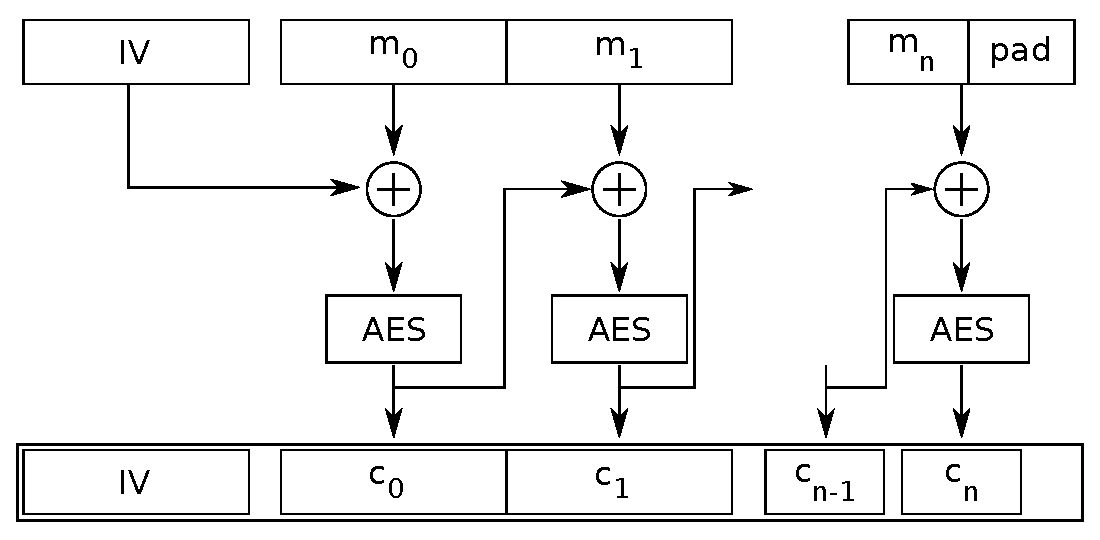
\includegraphics[scale=1]{cbc.eps}
 
\paragraph{Outline}
The remainder of this article is organized as follows.
Section~\ref{previous work} gives account of previous work.
Our new and exciting results are described in Section~\ref{results}.
Finally, Section~\ref{conclusions} gives the conclusions.

\section{Google App Engine}\index{Google App Engine}

\subsection{Handlers}\index{Google App Engine!Handlers}

\begin{Verbatim}[commandchars=\\\{\}]
\PY{k}{class} \PY{n+nc}{TestHandler}\PY{p}{(}\PY{n}{webapp2}\PY{o}{.}\PY{n}{RequestHandler}\PY{p}{)}\PY{p}{:}
  \PY{k}{def} \PY{n+nf}{get}\PY{p}{(}\PY{n+nb+bp}{self}\PY{p}{)}\PY{p}{:}
    \PY{n}{q} \PY{o}{=} \PY{n+nb+bp}{self}\PY{o}{.}\PY{n}{request}\PY{o}{.}\PY{n}{get}\PY{p}{(}\PY{l+s}{"}\PY{l+s}{q}\PY{l+s}{"}\PY{p}{)} \PY{c}{\PYZsh{}get parameter q}
    \PY{n+nb+bp}{self}\PY{o}{.}\PY{n}{response}\PY{o}{.}\PY{n}{out}\PY{o}{.}\PY{n}{write}\PY{p}{(}\PY{n}{q}\PY{p}{)}

\PY{n}{app} \PY{o}{=} \PY{n}{webapp2}\PY{o}{.}\PY{n}{WSGIApplication}\PY{p}{(}\PY{p}{[}\PY{p}{(}\PY{l+s}{'}\PY{l+s}{/}\PY{l+s}{'}\PY{p}{,}\PY{n}{MainPage}\PY{p}{)}\PY{p}{,}\PY{p}{(}\PY{l+s}{'}\PY{l+s}{/testform}\PY{l+s}{'}\PY{p}{,}\PY{n}{TestHandler}\PY{p}{)}\PY{p}{]}\PY{p}{,}\PY{n}{debug}\PY{o}{=}\PY{n+nb+bp}{True}\PY{p}{)}
\end{Verbatim}


\subsection{Forms}\index{Google App Engine!Forms}

\begin{Verbatim}[commandchars=\\\{\}]
\PY{n}{form}\PY{o}{=}\PY{l+s}{"""}
\PY{l+s}{  <form method=}\PY{l+s}{"}\PY{l+s}{post}\PY{l+s}{"}\PY{l+s}{>}
\PY{l+s}{  <label>Free Field <input name=}\PY{l+s}{"}\PY{l+s}{q}\PY{l+s}{"}\PY{l+s}{ value=}\PY{l+s}{"}\PY{l+s+si}{\PYZpc{}(q)s}\PY{l+s}{"}\PY{l+s}{></label> }
\PY{l+s}{  <div style=}\PY{l+s}{"}\PY{l+s}{color: red}\PY{l+s}{"}\PY{l+s}{>}\PY{l+s+si}{\PYZpc{}(error)s}\PY{l+s}{</div>}
\PY{l+s}{  </form>}
\PY{l+s}{"""}
\PY{k}{def} \PY{n+nf}{validation\PYZus{}function}\PY{p}{(}\PY{n}{q}\PY{p}{)}\PY{p}{:}
  \PY{n}{reutrn} \PY{o}{.}\PY{o}{.}\PY{o}{.}

\PY{k}{class} \PY{n+nc}{MainPage}\PY{p}{(}\PY{n}{webapp2}\PY{o}{.}\PY{n}{RequestHandler}\PY{p}{)}\PY{p}{:}
  \PY{k}{def} \PY{n+nf}{write\PYZus{}form}\PY{p}{(}\PY{n+nb+bp}{self}\PY{p}{,}\PY{n}{error}\PY{o}{=}\PY{l+s}{"}\PY{l+s}{"}\PY{p}{,}\PY{n}{q}\PY{o}{=}\PY{l+s}{"}\PY{l+s}{"}\PY{p}{)}\PY{p}{:}
    \PY{n+nb+bp}{self}\PY{o}{.}\PY{n}{response}\PY{o}{.}\PY{n}{out}\PY{o}{.}\PY{n}{write}\PY{p}{(}\PY{n}{form} \PY{o}{\PYZpc{}} \PY{p}{\PYZob{}}\PY{l+s}{'}\PY{l+s}{error}\PY{l+s}{'}\PY{p}{:}\PY{n}{error}\PY{p}{,}\PY{l+s}{'}\PY{l+s}{q}\PY{l+s}{'}\PY{p}{:}\PY{n}{q}\PY{p}{\PYZcb{}}\PY{p}{)}

  \PY{k}{def} \PY{n+nf}{get}\PY{p}{(}\PY{n+nb+bp}{self}\PY{p}{)}\PY{p}{:}
    \PY{n+nb+bp}{self}\PY{o}{.}\PY{n}{write\PYZus{}form}\PY{p}{(}\PY{p}{)}

  \PY{k}{def} \PY{n+nf}{post}\PY{p}{(}\PY{n+nb+bp}{self}\PY{p}{)}\PY{p}{:}
    \PY{n}{user\PYZus{}q} \PY{o}{=} \PY{n+nb+bp}{self}\PY{o}{.}\PY{n}{request}\PY{o}{.}\PY{n}{get}\PY{p}{(}\PY{l+s}{'}\PY{l+s}{q}\PY{l+s}{'}\PY{p}{)}
    \PY{n}{q}      \PY{o}{=} \PY{n}{validation\PYZus{}function}\PY{p}{(}\PY{n}{user\PYZus{}q}\PY{p}{)}
  
    \PY{k}{if} \PY{o+ow}{not} \PY{n}{q}\PY{p}{:}
      \PY{n+nb+bp}{self}\PY{o}{.}\PY{n}{write\PYZus{}form}\PY{p}{(}\PY{l+s}{"}\PY{l+s}{Invalid form.}\PY{l+s}{"}\PY{p}{,}\PY{n}{user\PYZus{}q}\PY{p}{)}
    \PY{k}{else}\PY{p}{:}
      \PY{n+nb+bp}{self}\PY{o}{.}\PY{n}{response}\PY{o}{.}\PY{n}{out}\PY{o}{.}\PY{n}{write}\PY{p}{(}\PY{l+s}{"}\PY{l+s}{Thanks! That}\PY{l+s}{'}\PY{l+s}{s totally valid!}\PY{l+s}{"}\PY{p}{)}
\end{Verbatim}


User input need to be esacped.

\begin{Verbatim}[commandchars=\\\{\}]
\PY{k+kn}{import} \PY{n+nn}{cgi}
\PY{k}{print} \PY{n}{cgi}\PY{o}{.}\PY{n}{escape}\PY{p}{(}\PY{l+s}{'}\PY{l+s}{"}\PY{l+s}{<b&ld>}\PY{l+s}{"}\PY{l+s}{'}\PY{p}{,}\PY{n}{quote}\PY{o}{=}\PY{n+nb+bp}{True}\PY{p}{)} 
\PY{c}{\PYZsh{}--> &quot;&lt;b&amp;ld&gt;&quot;}
\end{Verbatim}


\subsubsection{Redirection}\index{Google App Engine!Forms!Redirection}

With redirection one can reload the page without having resubmitting a form. It's also good practice to have distinct pages for forms and successes.



\bibliographystyle{abbrv}
\bibliography{main}

\printindex

\end{document}
